\documentclass[letterpaper,11pt]{article}

% -------------------------
% PAQUETES
% -------------------------
\usepackage[spanish]{babel}
\usepackage[utf8]{inputenc}
\usepackage[T1]{fontenc}
\usepackage{graphicx}
\usepackage{geometry}
\usepackage{array}
\usepackage{setspace}
\usepackage{titlesec}
\usepackage{enumitem}
\usepackage{amsmath}
\usepackage{amssymb}
\usepackage{float}
\usepackage{xcolor}
\usepackage{realboxes}
\geometry{margin=2.5cm}

\definecolor{lightgrey}{rgb}{0.95,0.95,0.95}
\newcommand{\code}[1]{\Colorbox{lightgrey}{\texttt{#1}}}

% -------------------------
% INICIO DOCUMENTO
% -------------------------

\begin{document}

\noindent
\begin{minipage}{0.39\textwidth}
    
\includegraphics[width=\linewidth]{logoUSM.png}
\end{minipage}
\hfill
\begin{minipage}{0.59\textwidth}
    \raggedleft
    \textbf{INGENIERÍA COMERCIAL}\\
    \textbf{2026-2}
\end{minipage}

\vspace{0.4cm}
\hrule
\vspace{0.1cm}

% -------------------------
% INFORMACIÓN CURSO
% -------------------------
\begin{center}
    {\Large \textbf{Control 2}}\\
    Econometría ICS-294\\
    II Semestre 2026\\
    \vspace{0.3cm}
    Profesor: Francisco Alfaro Medina
\end{center}

\textbf{Instrucciones:}

\begin{itemize}
    \item El trabajo deberá entregarse resuelto a mano.
    \item Cuide la presentación y la redacción de sus respuestas.
    \item Justifique sus respuestas e indique claramente los supuestos y
          valores críticos utilizados cuando corresponda.
\end{itemize}

\section{Preguntas}

Las preguntas y ejercicios están ordenados por tópico. En los contrastes,
utilice un nivel de significancia del 5\%, salvo que se indique lo contrario.

\subsection*{I. Interpretación y especificación de modelos}

\begin{enumerate}

\item Se estima el siguiente modelo para explicar el precio de una vivienda
    (\emph{PRICE}) en función de su superficie (\emph{SQFT}):
    \[
        \log(\text{PRICE})
        = 4{,}8 + 0{,}72\log(\text{SQFT}) + u,
    \]
    donde \texttt{PRICE} se mide en miles de pesos y \texttt{SQFT} en metros
    cuadrados.
    \begin{enumerate}[label=(\alph*)]
        \item Interprete el coeficiente estimado $\hat\beta_1=0{,}72$.
              ¿Qué concepto económico representa?
        \item Si la superficie aumenta en un 10\%, determine en cuánto cambia
              aproximadamente el precio.
    \end{enumerate}

\item El salario esperado, medido en logaritmos, en función de la experiencia
    laboral está dado por
    \[
        \widehat{\log(\text{salario})}
        = 2{,}5 + 0{,}25\,\texttt{exper}
        - 0{,}005\,\texttt{exper}^{2}.
    \]
    Determine el nivel de experiencia en el cual el retorno marginal de una
    unidad adicional de experiencia se anula. Interprete económicamente el
    resultado.

\end{enumerate}

\subsection*{II. MCO e inferencia sobre parámetros individuales}

\begin{enumerate}[resume]

\item Se estima el siguiente modelo para explicar el salario mensual
    (\emph{WAGE}) de 1.500 trabajadores en función de los años de educación
    (\emph{EDUC}), la experiencia laboral (\emph{EXPER}) y la residencia en
    zona rural (\emph{RURAL}, variable dicotómica):
    \[
        \log(\text{WAGE})
        =2{,}15+0{,}083\,\texttt{EDUC}
        +0{,}041\,\texttt{EXPER}
        -0{,}214\,\texttt{RURAL}+u.
    \]
    Los errores estándar de los estimadores son:
    \begin{center}
        \begin{tabular}{|c|c|}
            \hline
            \textbf{Variable} & \textbf{Error estándar}\\
            \hline
            \texttt{EDUC}  & 0{,}031\\
            \hline
            \texttt{EXPER} & 0{,}018\\
            \hline
            \texttt{RURAL} & 0{,}094\\
            \hline
        \end{tabular}
    \end{center}
    \begin{enumerate}[label=(\alph*)]
        \item Plantee las hipótesis para evaluar si la educación tiene un
              efecto positivo y significativo sobre el salario. Indique si el
              contraste es unilateral o bilateral y justifique.
        \item Calcule los estadísticos $t$ para \texttt{EDUC} y \texttt{RURAL}.
              Concluya si cada variable es individualmente significativa e
              interprete los resultados.
        \item Para \texttt{EXPER}, el valor-$p$ reportado es $0{,}038$.
              Interprete este valor-$p$ y determine si cambiaría su conclusión
              al utilizar un nivel de significancia del 1\%.
    \end{enumerate}

\item Utilizando una base de datos de 4.137 alumnos universitarios, se estimó
    por MCO la ecuación
    \[
        \widehat{\texttt{colgpa}}
        =2{,}000-0{,}5000\,\texttt{hsperc}
        +0{,}0100\,\texttt{sat},
    \]
    con $R^2=0{,}273$. La variable \texttt{colgpa} es el promedio de notas
    universitarias, \texttt{hsperc} es el percentil de graduación de enseñanza
    media y \texttt{sat} es el puntaje combinado de admisión. Considere
    \[
        (X'X)^{-1}=
        \begin{bmatrix}
            8{,}5 & 0{,}19 & -0{,}11\\
            0{,}19 & 0{,}5 & -0{,}02\\
            -0{,}11 & -0{,}02 & 0{,}04
        \end{bmatrix},
        \qquad \widehat{\sigma}^{2}=0{,}01.
    \]
    \begin{enumerate}[label=(\alph*)]
        \item Calcule el promedio de calificaciones predicho cuando
              \texttt{hsperc}$=20$ y \texttt{sat}$=900$.
        \item Explique por qué es razonable que el coeficiente de
              \texttt{hsperc} sea negativo. Contraste la hipótesis de que el
              coeficiente poblacional asociado a \texttt{hsperc} es negativo.
              Use $t_{0{,}05;\,4134}=1{,}645$.
        \item Contraste la hipótesis de que un aumento de un punto en
              \texttt{hsperc} se compensa exactamente con un aumento de diez
              puntos en \texttt{sat}. En términos del modelo, la hipótesis es
              $H_0:\beta_1+10\beta_2=0$. Calcule el estadístico correspondiente
              e interprete su resultado.
    \end{enumerate}

\end{enumerate}

\subsection*{III. Restricciones lineales y pruebas conjuntas}

\begin{enumerate}[resume]

\item Dada una muestra de 353 jugadores de béisbol, se estiman los siguientes modelos
    para el logaritmo del salario por hora:
    \[
    \begin{aligned}
        \text{Modelo 1:}\quad
        \log(\text{salario})={}&\beta_0+\beta_1\texttt{years}
        +\beta_2\texttt{gamesyr}+\beta_3\texttt{hrunsyr}
        +\beta_4\texttt{rbisyr}+v,\\
        &n=353,\qquad R_1^2=0{,}627,
    \end{aligned}
    \]
    y
    \[
    \begin{aligned}
        \text{Modelo 2:}\quad
        \log(\text{salario})={}&\gamma_0+\gamma_1\texttt{years}
        +\gamma_2\texttt{gamesyr}+\varepsilon,\\
        &n=353,\qquad R_2^2=0{,}597.
    \end{aligned}
    \]
    \begin{enumerate}[label=(\alph*)]
        \item Contraste en el Modelo 1
              $H_0:\beta_3=\beta_4=0$ frente a la alternativa de que al
              menos uno de estos parámetros sea distinto de cero. Identifique
              los modelos restringido y no restringido.
        \item Contraste en el Modelo 1 la significancia global:
              $H_0:\beta_1=\beta_2=\beta_3=\beta_4=0$. Identifique el modelo
              restringido y calcule el estadístico $F$.
        \item Use $F_{0{,}05}^{(2,348)}\approx3{,}02$ y
              $F_{0{,}05}^{(4,348)}\approx2{,}40$ para tomar sus decisiones.
    \end{enumerate}

\item Demuestre que, para contrastar $j$ restricciones lineales mediante un
    modelo restringido ($R$) y uno no restringido ($UR$), el estadístico $F$
    puede escribirse como
    \[
        \widehat F
        =\frac{SSR_R-SSR_{UR}}{SSR_{UR}}
         \frac{n-k-1}{j}
        =\frac{R^2_{UR}-R^2_R}{1-R^2_{UR}}
         \frac{n-k-1}{j}.
    \]
    Explique qué representan $SSR_R$, $SSR_{UR}$, $R_R^2$ y $R_{UR}^2$.

\item Se tiene el modelo
    \[
        y=\beta_0+\beta_1x_1+\beta_2x_2+\beta_3x_3+u,
    \]
    estimado con 150 observaciones. Se obtiene
    \[
        \widehat{\boldsymbol\beta}
        =\begin{bmatrix}5{,}5\\10{,}1\\1{,}2\\2{,}1\end{bmatrix},
        \qquad
        \widehat{\sigma}^{2}=1{,}5,
    \]
    y
    \[
        (X'X)^{-1}=
        \begin{bmatrix}
            1{,}1 & 0{,}3 & 0{,}4 & 0{,}3\\
            0{,}3 & 2{,}2 & 0{,}25 & 1{,}3\\
            0{,}4 & 0{,}25 & 0{,}27 & -0{,}16\\
            0{,}3 & 1{,}3 & -0{,}16 & 1{,}3
        \end{bmatrix}.
    \]
    \begin{enumerate}[label=(\alph*)]
        \item Plantee las hipótesis para contrastar $3\beta_2=2\beta_3$.
        \item Calcule el estadístico $t$ y determine si se rechaza la hipótesis
              nula al 5\%.
        \item Construya un intervalo de confianza al 95\% para
              $3\beta_2-2\beta_3$ e interprételo.
    \end{enumerate}

\end{enumerate}

\newpage
\section{Formulario}

\begin{itemize}
    \item Estimador de MCO:
    \[
        \widehat{\boldsymbol\beta}
        =(X'X)^{-1}X'y.
    \]

    \item Para un modelo con constante:
    \[
        SST=\sum_{i=1}^{n}(y_i-\bar y)^2,\qquad
        SSE=\sum_{i=1}^{n}(\widehat y_i-\bar y)^2,\qquad
        SSR=\sum_{i=1}^{n}\widehat u_i^2.
    \]
    Aquí, $SST=SSE+SSR$.

    \item Coeficiente de determinación:
    \[
        R^2=\frac{SSE}{SST}=1-\frac{SSR}{SST}.
    \]

    \item Estadístico $t$ para $H_0:\beta_j=a_j$:
    \[
        t=\frac{\widehat\beta_j-a_j}{se(\widehat\beta_j)}.
    \]

    \item Intervalo de confianza de $100(1-\alpha)\%$ para $\beta_j$:
    \[
        \widehat\beta_j\pm t_{\alpha/2,\,n-k-1}
        \,se(\widehat\beta_j).
    \]

    \item Para una combinación lineal $c'\beta$:
    \[
    \begin{aligned}
        se(c'\widehat\beta)
        &=\sqrt{c'\widehat{\operatorname{Var}}(\widehat\beta)c},\\
        t&=\frac{c'\widehat\beta-r}{se(c'\widehat\beta)}.
    \end{aligned}
    \]

    \item Varianza de una combinación lineal:
    \[
        \operatorname{Var}(aA+bB)
        =a^2\operatorname{Var}(A)+b^2\operatorname{Var}(B)
        +2ab\operatorname{Cov}(A,B).
    \]

    \item Estadístico $F$ para $j$ restricciones lineales:
    \[
        \widehat F
        =\frac{SSR_R-SSR_{UR}}{SSR_{UR}}
        \frac{n-k-1}{j}
        =\frac{R^2_{UR}-R^2_R}{1-R^2_{UR}}
        \frac{n-k-1}{j}.
    \]
    El modelo no restringido contiene todas las variables; el modelo
    restringido impone las restricciones de $H_0$.

    \item En modelos log-log, $\beta_j$ es una elasticidad: un aumento de
    1\% en $x_j$ se asocia aproximadamente con un cambio de $\beta_j\%$ en
    $y$. En un modelo log-nivel, un aumento de una unidad en $x_j$ se asocia
    aproximadamente con un cambio de $100\beta_j\%$ en $y$.

    \item Valores críticos usuales para muestras grandes:
    \[
        t_{0{,}95}=1{,}645,\qquad t_{0{,}975}=1{,}96.
    \]
\end{itemize}

\begin{figure}[H]
    \centering
    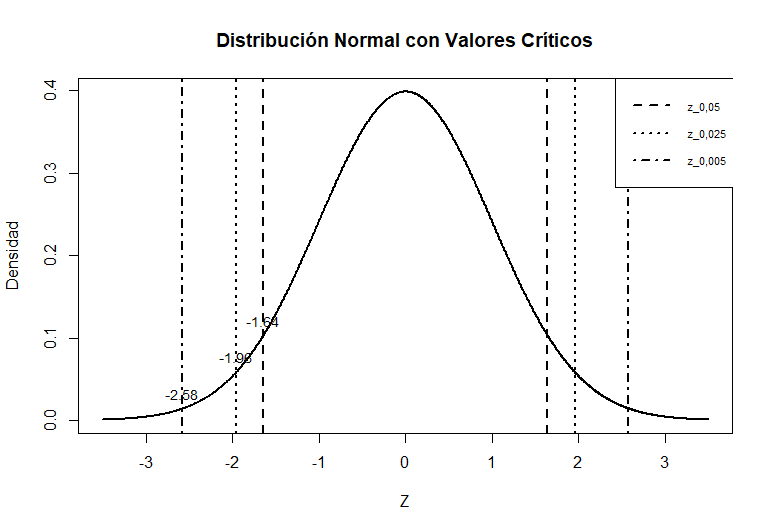
\includegraphics[width=0.9\linewidth]{normal_critic.png}
\end{figure}

\end{document}
